\documentclass[11pt,twoside,reqno]{amsart}
\usepackage{amssymb, amsmath, enumerate, palatino, hyperref}
\usepackage[normalem]{ulem}
%\usepackage{fullpage}
\usepackage[margin=1in]{geometry}
\usepackage[T1]{fontenc}
\renewcommand{\labelitemi}{\guillemotright}
\usepackage{mathrsfs}
%--------------------------------
% Kees' imports
%--------------------------------
\usepackage{physics}
\usepackage{tensor}
\usepackage{mathtools}
\usepackage{xcolor}
\usepackage{siunitx}
\usepackage{empheq}
\usepackage{tensor}


\theoremstyle{plain}
\newtheorem{prop}{Proposition}%[section]
\newtheorem{lemma}[prop]{Lemma}
\newtheorem{thm}[prop]{Theorem}
\newtheorem{obs}[prop]{Observation}
\newtheorem{app}[prop]{Application}
\newtheorem*{MainThm}{Main Theorem}
\newtheorem{cor}[prop]{Corollary}
\newtheorem{conj}[prop]{Conjecture}
\theoremstyle{remark}
\newtheorem{rmk}[prop]{Remark}
\theoremstyle{definition}
\newtheorem{prob}{Problem}
\newtheorem{bonus}[prop]{Bonus Problem}
\theoremstyle{remark}
\newtheorem{exc}{Exercise}
\newtheorem*{soln}{Solution}
\theoremstyle{definition}
\newtheorem{ex}[prop]{Example}
\theoremstyle{definition}
\newtheorem{defn}[prop]{Definition}

\newcommand{\RR}{\mathbb{R}}
\newcommand{\ZZ}{\mathbb{Z}}
\newcommand{\CC}{\mathbb{C}}
\newcommand{\NN}{\mathbb{N}}
\newcommand{\QQ}{\mathbb{Q}}

\newcommand{\Aut}{\operatorname{Aut}}

\newcommand{\defeq}{:=}

\renewcommand{\Re}{\operatorname{Re}}

%--------------------------------
% Kees' commands
%--------------------------------
\makeatletter
\newcommand{\subalign}[1]{%
  \vcenter{%
    \Let@ \restore@math@cr \default@tag
    \baselineskip\fontdimen10 \scriptfont\tw@
    \advance\baselineskip\fontdimen12 \scriptfont\tw@
    \lineskip\thr@@\fontdimen8 \scriptfont\thr@@
    \lineskiplimit\lineskip
    \ialign{\hfil$\m@th\scriptstyle##$&$\m@th\scriptstyle{}##$\hfil\crcr
      #1\crcr
    }%
  }%
}
\makeatother

\newcommand{\allspace}{{\substack{\text{all}\\\text{space}}}}

\newcommand{\DD}{\mathbb{D}}
\renewcommand{\AA}{\mathbb{A}}
\newcommand{\VV}{\mathbb{V}}
\newcommand{\LL}{\mathbb{L}}
\newcommand{\BB}{\mathbb{B}}
\renewcommand{\SS}{\mathbb{S}}
\newcommand{\HH}{\mathbb{H}}

\renewcommand{\l}{\ell}

\newcommand{\PB}{\mathrm{PB}}

\newcommand{\cL}{\mathcal{L}}
\newcommand{\cE}{\mathcal{E}}
\newcommand{\cH}{\mathcal{H}}
\newcommand{\cC}{\mathcal{C}}
\newcommand{\cA}{\mathcal{A}}
\newcommand{\cI}{\mathcal{I}}
\newcommand{\cM}{\mathcal{M}}
\newcommand{\cO}{\mathcal{O}}

\newcommand{\sgn}{\mathrm{sgn}}

\newcommand{\LIPS}{\mathrm{LIPS}}
\newcommand{\zcut}{z_\mathrm{cut}}

\newcommand{\Ei}{\mathrm{Ei}}
\newcommand{\Li}{\mathrm{Li}}

\def\beq#1\eeq{\begin{equation}#1\end{equation}}
\def\bal#1\eal{\begin{align}#1\end{align}}

\title{Groomed heavy hemisphere mass to first order, collinear limit}
\author{Kees Benkendorfer}
\date{3 December 2020}

\begin{document}
\maketitle

\tableofcontents

\section{Setup}

\subsection{Heavy jet mass}\label{sec: mass}

	Now we wish to calculate the mass of the heavy hemisphere in an $e^+ e^- \to q\bar q g$ event after mMDT grooming, assuming a collinear gluon emission. If $E_h$ is the energy of the heavy hemisphere and $m_h$ is the mass, then the observable of interest is \cite{larkoski_improving_2020}
	\begin{equation}
		\rho = \qty(\frac{m_h}{E_h})^2.
	\end{equation}
	In the collinear limit, $E_h \to Q/2$ with $Q$ (shorthand for $\sqrt{Q^2}$) the energy of the event. To compute $m_h$, we introduce the phase space variables
	\begin{equation}
		x_i = \frac{2 p_i \cdot Q}{Q^2}
	\end{equation}
	with $p_i$ the four-momentum of the $i$-th particle and $Q$ the total four-momentum (not to be confused with $Q$ the total energy). Let $x_3$ be the energy fraction of the gluon and $x_1$ be the energy fraction of the quark. 

	We assume that the gluon is collinear with the quark (we will later multiply our result by $2$ to account for the case where the gluon is collinear to the antiquark) and introduce the gluon's hemisphere energy fraction
	\begin{equation}
		z = \frac{x_3}{x_1 + x_3} = x_3
	\end{equation}
	where we have noted that, in the collinear limit, $x_1 + x_3 \to 1$. Notice that
	\begin{equation}
		1 - z = \frac{x_1}{x_1 + x_3} = x_1
	\end{equation}
	is the quark's hemisphere energy fraction. This is equivalent to the assumption that the quark four-momentum $p_1$ and gluon four-momentum $k$ are collinear along some vector $\bar p_1$:
	\begin{align}
		k &= z \bar p_1 & p_q &= (1 - z)\bar p_1.
	\end{align}

	Now notice that
	\begin{equation}
		1 - x_2 = \frac{Q^2 - 2 p_2 \cdot Q}{Q^2} = \frac{2 p_1 \cdot k}{Q^2} = \frac{x_1 x_3}{2}\qty(1 - \cos \theta)
	\end{equation}
	where $\theta$ is the angle between the quark and gluon. In the collinear limit $\theta \ll 1$, this means that
	\begin{equation}
		\frac{2 p_1 \cdot k}{Q^2} = \frac{x_1 x_3}{4}\theta^2 = \frac{z(1 - z)}{4}\theta^2.
	\end{equation}
	Then the heavy hemisphere mass is
	\begin{equation}
		m_h = (p_1 + k)^2 = 2p_1 \cdot k = \frac{z(1 - z)}{4}\theta^2 Q^2.
	\end{equation}
	This means that
	\begin{equation}
		\rho = z(1 - z)\theta^2.
	\end{equation}
	This suggests a measurement term of
	\begin{equation}\label{eq:measurement}
		\delta(\rho - z(1 - z)\theta^2) = \frac{1}{z(1 - z)} \delta\qty(\theta^2 - \frac{\rho}{z(1 - z)}).
	\end{equation}


\subsection{Grooming}

	The heavy hemisphere only passes the mMDT groomer if \cite{kardos_two-_2020}
	\begin{equation}
		\frac{\min[E_1, E_3]}{E_1 + E_3} > \zcut
	\end{equation}
	for some fixed $\zcut$. This means
	\begin{equation}
		\min[x_1, x_3] = \min[z, 1 - z] > \zcut.
	\end{equation}
	Thus, we must introduce the grooming term
	\begin{equation}\label{eq: grooming}
		\Theta(\min[z, 1 - z] - \zcut)
	\end{equation}
	into our calculation.
	

\subsection{Matrix element}

	The matrix element for $e^+ e^- \to q \bar q g$ is \cite{larkoski_improving_2020}
	\begin{equation}\label{eq:matrix element}
		\abs{\cM}^2 = 4 \pi \alpha_s \sigma_0 C_F \frac{x_1^2 + x_2^2}{(1 - x_1)(1 - x_2)}
	\end{equation}
	where $4\pi\alpha_s$ is the strong coupling (squared), $\sigma_0$ is the cross section for $e^+ e^- \to q \bar q$, and $C_F$ is the quadratic Casimir of the fundamental representation of color. Under the change of variables introduced in Sec.\ \ref{sec: mass}, this reduces (after introducing the appropriate Jacobian factor) to the collinear splitting function
	\begin{equation}
		\abs{\cM}^2 = 4 \pi \alpha_s \sigma_0 C_F \frac{1 + (1 - z)^2}{z \theta^2}.
	\end{equation}


\subsection{Lorentz-invariant phase space}

	Working in $d = 4 - 2\epsilon$ dimensions, the phase space integral with matrix element {\color{red}\textbf{[from Andrew's notes]}} is
	\begin{equation}
	\begin{aligned}
		\frac{4\pi}{\alpha_s C_F}\frac{1}{\sigma_0} \sigma = \frac{1}{\sqrt{\pi} \, \Gamma(\frac{1}{2} - \epsilon)} \qty(\frac{4 \mu^2}{Q^2})^\epsilon \int_0^1 dz \int_0^\infty d\theta^2 \int_0^{2\pi} d\phi &\sin^{-2\epsilon}\phi \, \qty(\theta^2)^{-1 - \epsilon} z^{-2\epsilon} (1 - z)^{-2\epsilon} \\
			&\times \qty(\frac{1 + (1 - z)^2}{z} - \epsilon z).
	\end{aligned}
	\end{equation}
	Here, $\mu$ is a mass scale introduced to ensure the proper dimensionality and $\phi$ is the azimuthal angle. Notice that the matrix element is slightly modified under the dimensional regularization prescription.

	Introducing the measurement and grooming terms of Eqs.\ \ref{eq:measurement} and \ref{eq: grooming}, the differential cross section in $\rho$ is
	\begin{equation}\label{eq:cross section integral}
	\boxed{
	\begin{aligned}
		\frac{4\pi}{\alpha_s C_F}\frac{1}{\sigma_0} \frac{d\sigma}{d\rho} = \frac{1}{\sqrt{\pi} \, \Gamma(\frac{1}{2} - \epsilon)} \qty(\frac{4 \mu^2}{Q^2})^\epsilon \int_0^{\pi} d\phi\, & \sin^{-2\epsilon}\phi \int_0^1 dz \int_0^\infty d\theta^2  \, \qty(\theta^2)^{-1 - \epsilon} z^{-2\epsilon} (1 - z)^{-2\epsilon} \\
			&\times \qty(\frac{1 + (1 - z)^2}{z} - \epsilon z) \frac{1}{z(1 - z)}\delta\qty(\theta^2 - \frac{\rho}{z(1 - z)})\\
			&\times \Theta(\min[z, 1 - z] - \zcut).
	\end{aligned}
	}
	\end{equation}


\section{Integration}

	Integrating first in $\theta^2$, we find
	\begin{equation}
	\begin{aligned}
		\frac{4\pi}{\alpha_s C_F}\frac{1}{\sigma_0} \frac{d\sigma}{d\rho} = \frac{1}{\sqrt{\pi} \, \Gamma(\frac{1}{2} - \epsilon)} \qty(\frac{4 \mu^2}{Q^2})^\epsilon \int_0^{\pi} d\phi\, \sin^{-2\epsilon}\phi \int_0^1 dz\, &\frac{1}{\rho^{1 + \epsilon}} \frac{1}{z^\epsilon (1 - z)^\epsilon} \qty(\frac{1 + (1 - z)^2}{z} - \epsilon z) \\
			&\times \Theta(\min[z, 1 - z] - \zcut).
	\end{aligned}
	\end{equation}
	The $\phi$ integral can be done immediately as well:
	\begin{equation}
		\int_0^\pi d\phi \,\sin^{-2\epsilon}\phi = \frac{\sqrt{\pi}\,\Gamma\qty(\frac{1}{2} - \epsilon)}{\Gamma(1 - \epsilon)}.
	\end{equation}
	The Heaviside function can be satisfied by ensuring that
	\begin{equation}
		\zcut < z < 1 - \zcut,
	\end{equation}
	so
	\begin{equation}
		\int_0^1 dz\, \Theta(\min[z, 1 - z] - \zcut) = \int_{\zcut}^{1 - \zcut}dz.
	\end{equation}
	Thus, the cross section is
	\begin{equation}
		\frac{4\pi}{\alpha_s C_F}\frac{1}{\sigma_0} \frac{d\sigma}{d\rho} = \qty(\frac{4\mu^2}{Q^2})^\epsilon \frac{1}{\Gamma(1 - \epsilon)}\frac{1}{\rho^{1+\epsilon}} \int_{\zcut}^{1 - \zcut} \frac{1}{z^\epsilon (1 - z)^\epsilon} \qty(\frac{1 + (1 - z)^2}{z} - \epsilon z).
	\end{equation} 
	Notice that no cusp will emerge from this integral. This is a result of the particular radiative modes we pick out by considering the collinear limit, as revealed by power counting arguments. Let $z_i$ be the energy fraction of the $i$-th emission in the hemisphere, with angle $\theta_i$ from the hard quark and $\theta_{ij}$ the angle between emissions $i$ and $j$. Then
	\begin{equation}
		\rho \simeq \sum_{i,j}z_i z_j\theta_{ij}^2.
	\end{equation}
	The cusp occurs around $\rho \sim \zcut \ll 1$, which would require $z_i \ll 1$. Around the cusp, we want $z_i$ to be sensitive to both $\rho$ \textit{and} $\zcut$, so we also have $z_i \sim \zcut$. Moreover, the leading contribution from emission $i$ comes with its interaction with the hard quark, since $z_i z_j$ is largest when $z_j$ is hard. Therefore, we expect $\rho \sim z_i \theta_i^2$. But then
	\begin{equation}
		\rho \sim \zcut \theta_i^2 \sim \zcut,
	\end{equation}
	so $\theta_i \sim 1$. Thus, emissions that contribute to the cusp must be \textit{soft and wide-angle}. When we consider the collinear limit, we are moving out of the cusp region.

	Returning to the integration a hand, the final integral is difficult to do directly, so we will first expand in $\epsilon$. To first order in $\epsilon$, we have
	\begin{equation}
		\frac{1}{z^\epsilon (1 - z)^\epsilon} \qty(\frac{1 + (1 - z)^2}{z} - \epsilon z) = \frac{2 - 2z + z^2}{z} - \epsilon \qty(\frac{2 - 2z + z^2}{z}\log(z(1 - z)) + z) + \cO(\epsilon^2).
	\end{equation}
	The corresponding integrals are
	\begin{equation}
		\int_{\zcut}^{1 - \zcut} dz\, \frac{2 - 2z + z^2}{z} = -\frac{3}{2} + 3\zcut + 2\log(\frac{1 - \zcut}{\zcut})
	\end{equation}
	and
	\begin{equation}
	\begin{aligned}
		\int_{\zcut}^{1 - \zcut} dz\, \qty(\frac{2 - 2z + z^2}{z}\log(z(1 - z)) + z) &= 2 \mathrm{Li}_2(\zcut) -2 \mathrm{Li}_2(1-\zcut) - 7 \zcut - \log^2\zcut \\
			&\quad + \log \zcut\qty(3\zcut + \frac{7}{2})  +\frac{7}{2}  \\
			&\quad +\log (1-\zcut) (3 \zcut + \log (1-\zcut )-3).
	\end{aligned}
	\end{equation}
	where $\Li_n$ is the polylogarithm function
	\begin{equation}
		\Li_n(x) = \sum_{k = 1}^\infty \frac{x^k}{k^n}.
	\end{equation}
	Thus
	\begin{equation}
	\begin{aligned}
		\int_{\zcut}^{1 - \zcut} dz\,\frac{1}{z^\epsilon (1 - z)^\epsilon} &\qty(\frac{1 + (1 - z)^2}{z} - \epsilon z) = -\frac{3}{2} + 3\zcut + 2\log(\frac{1 - \zcut}{\zcut}) \\
			&+ \epsilon \bigg[ 2 \mathrm{Li}_2(\zcut) -2 \mathrm{Li}_2(1-\zcut) - 7 \zcut - \log^2\zcut \\
			&\quad + \log \zcut\qty(3\zcut + \frac{7}{2}) + \frac{7}{2}  \\
			&\quad +\log (1-\zcut) (3 \zcut + \log (1-\zcut )-3) \bigg] + \cO(\epsilon^2).
	\end{aligned}
	\end{equation}
	We can expand $1/\rho^{1 + \epsilon}$ using a plus-function expansion \cite{lazopoulos_qcd_2007}:
	\begin{equation}
		\frac{1}{\rho^{1 + \epsilon}} = -\frac{1}{\epsilon}\delta(\rho) + \qty[\frac{1}{\rho}]_+ + \cO(\epsilon).
	\end{equation}
	The prefactor takes the form
	\begin{equation}
		\frac{1}{\Gamma(1 - \epsilon)} \qty(\frac{4 \mu^2}{Q^2})^\epsilon = 1 + \epsilon\log(\frac{4\mu^2}{Q^2}) + \cO(\epsilon^2).
	\end{equation}
	Putting everything together, we find
	\begin{equation}\label{eq:collinear result}
	\boxed{
	\begin{aligned}
		\frac{4\pi}{\alpha_s C_F}\frac{1}{\sigma_0}\frac{d\sigma}{d\rho} 
		&= -\frac{1}{\epsilon} \qty(-\frac{3}{2} + 3\zcut + 2\log(\frac{1 - \zcut}{\zcut}))\delta(\rho) \\
			&\quad - \delta(\rho)\bigg[2\log(\frac{4\mu^2}{Q^2}) + 2 \mathrm{Li}_2(\zcut) -2 \mathrm{Li}_2(1-\zcut) - 7 \zcut - \log^2\zcut \\
			&\qquad\qquad\qquad + \log \zcut\qty(3\zcut + \frac{7}{2}) + \frac{7}{2}  \\
			&\qquad\qquad\qquad +\log (1-\zcut) (3 \zcut + \log (1-\zcut )-3)\bigg] \\
			&\quad + \qty[\frac{1}{\rho}]_+ \qty[-\frac{3}{2} + 3\zcut + 2\log(\frac{1 - \zcut}{\zcut}) ] + \cO(\epsilon).
	\end{aligned}
	}
	\end{equation}

\section{Laplace transform}

	{\color{red}\textbf{[TODO]}}

\section{Soft and collinear limit}

	Now we take the soft and collinear limit. This can be achieved by starting in the collinear limit and taking $z \ll 1$. The cross section is then given by a correspondingly modified version of Eq.\ \ref{eq:cross section integral}:
	\begin{equation}
	\boxed{
	\begin{aligned}
		\frac{4\pi}{\alpha_s C_F}\frac{1}{\sigma_0} \frac{d\sigma}{d\rho} = \frac{2}{\Gamma(1 - \epsilon)} \qty(\frac{4 \mu^2}{Q^2})^\epsilon \int_0^\infty dz \int_0^\infty d\theta^2  \, \qty(\theta^2)^{-1 - \epsilon}\frac{1}{z^{2 + 2\epsilon}}\,\delta\qty(\theta^2 - \frac{\rho}{z})\Theta(z - \zcut).
	\end{aligned}
	}
	\end{equation}
	The upper bound on the $z$ integral has been taken from $1 \to \infty$ because in the $z \ll 1$ limit, the integral should not depend on the particular upper bound {\color{red}\textbf{[This seems like sketchy reasoning\dots is it right? Is there a more rigorous way to prove it? It's necessary in order to get a finite result in the end]}}. Another simplification came in the mMDT grooming term, where we have taken $\min[z, 1 - z] \to \min[z, 1] \to z$. Note also that we have already performed the $\phi$ integral.

	Performing the remaining integrals, we have
	\begin{align}
		\frac{4\pi}{\alpha_s C_F}\frac{1}{\sigma_0} \frac{d\sigma}{d\rho} &= \frac{2}{\Gamma(1 - \epsilon)} \qty(\frac{4 \mu^2}{Q^2})^\epsilon \frac{1}{\rho^{1+\epsilon}} \int_{\zcut}^\infty dz \,\frac{1}{z^{1 + \epsilon}} \\
		&=  \frac{2}{\Gamma(1 - \epsilon)} \qty(\frac{4 \mu^2}{Q^2})^\epsilon \frac{1}{\rho^{1+\epsilon}} \frac{\zcut^{-\epsilon}}{\epsilon}.
	\end{align}
	The prefactor can be expanded in $\epsilon$ as
	\begin{equation}
	\begin{aligned}
		\frac{2}{\Gamma(1 - \epsilon)} \qty(\frac{4 \mu^2}{Q^2})^\epsilon \frac{\zcut^\epsilon}{\epsilon} &= \frac{2}{\epsilon } + 2 \left(\log \left(\frac{4 \mu ^2}{Q^2}\right)-\log\zcut\right) \\
			&\quad+ \epsilon  \bigg[\log^2 \qty(\frac{4\mu ^2}{Q^2})  - 2 \log \zcut \log(\frac{4 \mu^2}{Q^2}) + \log ^2\zcut - \frac{\pi ^2}{6}+4 \log ^2(2) \bigg] \\
			&\quad+ \cO\left(\epsilon ^2\right).
  	\end{aligned}
	\end{equation}
	Using the usual plus-function expansion
	\begin{equation}
		\frac{1}{\rho^{1 + \epsilon}} = -\frac{1}{\epsilon}\delta(\rho) + \qty[\frac{1}{\rho}]_+ - \epsilon\qty[\frac{\log\rho}{\rho}]_+ + \cO(\epsilon^2),
	\end{equation}
	we therefore find
	\begin{equation}\label{eq:soft collinear result}
	\boxed{
	\begin{aligned}
		\frac{4\pi}{\alpha_s C_F}\frac{1}{\sigma_0} \frac{d\sigma}{d\rho} &= -\frac{2}{\epsilon^2}\delta(\rho) + \frac{2}{\epsilon} \qty(\qty[\frac{1}{\rho}]_+ - \qty[\log(\frac{4\mu^2}{Q^2}) - \log\zcut]\delta(\rho)) \\
			&\quad+ 2\qty[\frac{1}{\rho}]_+ \left(\log \left(\frac{4 \mu ^2}{Q^2}\right)-\log\zcut\right) - 2\qty[\frac{\log\rho}{\rho}]_+ \\
			&\quad- \bigg[\log^2 \qty(\frac{4\mu ^2}{Q^2})  - 2 \log \zcut \log(\frac{4 \mu^2}{Q^2}) + \log ^2\zcut - \frac{\pi ^2}{6}+4 \log ^2(2) \bigg]\delta(\rho) \\
			&\quad+ \cO(\epsilon).
	\end{aligned}
	}
	\end{equation}

\section{Combining soft and collinear results}
	
	To achieve a finite result, we need to add together the contributions from all of phase space:
	\begin{equation}
		\frac{d\sigma}{d\rho} = \frac{d\sigma^\text{soft}}{d\rho} + \frac{d\sigma^\text{collinear}}{d\rho} - \frac{d\sigma^\text{soft-collinear}}{d\rho}.
	\end{equation}
	The soft-collinear contributions are subtracted at the end to compensate for over-counting: these are included both in the soft term and in the collinear term.

\subsection{Soft results}
	{\color{black}\,}

	{\color{red}[Initially, I think I made a mistake with the soft contribution. I said 
	\begin{equation}
		d^{d-2}k_\perp = k_\perp^{d-3} dk_\perp d\Omega_{d-3},
	\end{equation}
	but perhaps this should have been
	\begin{equation}
		d^{d-2}k_\perp = k_\perp^{d-3} dk_\perp d\Omega_{d-2}.
	\end{equation}
	Thus, when integrating over the solid angle, I got
	\begin{equation}
		\Omega_{d-3} = \frac{2\pi^{(d-3)/2}}{\Gamma\qty(\frac{d - 3}{2})} = \frac{2\sqrt{\pi}}{\pi^\epsilon \Gamma(\frac{1}{2} - \epsilon)}
	\end{equation}
	instead of 
	\begin{equation}
		\Omega_{d-2} = \frac{2\pi^{(d-2)/2}}{\Gamma\qty(\frac{d - 2}{2})} = \frac{2\pi}{\pi^\epsilon \Gamma(1 - \epsilon)}.
	\end{equation}
	Therefore, we should actually take
	\begin{equation}
		\frac{1}{8\pi^{5/2}\Gamma(\frac{1}{2} - \epsilon)} \to \frac{1}{8\pi^2 \Gamma(1 - \epsilon)}.
	\end{equation}
	]}

	Recall that the soft contribution is {\color{red}\textbf{[there is a missing factor of $1/4$ from the soft calculation\dots I will include it now]}}
	\begin{equation}
	\begin{aligned}
		\frac{4\pi}{\alpha_s C_F}\frac{1}{\sigma_0} \frac{d\sigma^{\text{soft}}}{d\rho} = 
		\frac{Q \mu^{2\epsilon}}{2\Gamma(1 - \epsilon)} \qty(\frac{4}{Q \rho})^{1 + \epsilon} \frac{1}{\epsilon} \qty[ \Theta(\rho - 2\zcut) \qty(\frac{4}{Q\rho})^\epsilon + \Theta(2\zcut - \rho) \qty(Q\zcut - \frac{Q\rho}{4})^{-\epsilon} ].
	\end{aligned}
	\end{equation}
	For the first term,
	\begin{equation}
	\begin{aligned}
		\frac{Q \mu^{2\epsilon}}{2\Gamma(1 - \epsilon)} \qty(\frac{4}{Q})^{1 + 2\epsilon} \frac{1}{\epsilon} \frac{1}{\rho^\epsilon} &= \frac{2}{\epsilon} + 2\log(\frac{16\mu^2}{Q^2\rho}) \\
		&\qquad+ \epsilon\qty[-\frac{\pi^2}{6} + 16 \log^2 2 + \log(\frac{16^2 \mu^2}{Q^2 \rho})\log(\frac{\mu^2}{Q^2\rho})] + \cO(\epsilon^2),
	\end{aligned}
	\end{equation}
	Notice that we don't need the plus-function expansion of $1/\rho^\epsilon$ because $\rho$ never approaches $0$. The plus-function expansion of $1/\rho^{1+\epsilon}$ is, on the other hand, is
	\begin{equation}
		\frac{1}{\rho^{1+\epsilon}} = -\frac{1}{\epsilon}\delta(\rho) + \qty[\frac{1}{\rho}]_+ - \epsilon\qty[\frac{\log\rho}{\rho}]_+ + \cO(\epsilon),
	\end{equation}
	so the full term is
	\begin{equation}
	\begin{aligned}
		\frac{Q \mu^{2\epsilon}}{2\Gamma(1 - \epsilon)} \qty(\frac{4}{Q})^{1 + 2\epsilon} \frac{1}{\epsilon} \frac{1}{\rho^\epsilon}\frac{1}{\rho^{1+\epsilon}} &= -\frac{2}{\epsilon^2}\delta(\rho) + \frac{1}{\epsilon}\qty[2\qty[\frac{1}{\rho}]_+ - 2\log(\frac{16\mu^2}{Q^2\rho})\delta(\rho)] \\
			&\quad -2\qty[\frac{\log\rho}{\rho}]_+ + \qty[\frac{\pi^2}{6} - 16 \log^2 2 - \log(\frac{16^2\mu^2}{Q^2\rho})\log(\frac{\mu^2}{Q^2\rho})]\delta(\rho) \\
			&\quad+ 2\log(\frac{16\mu^2}{Q^2\rho})\qty[\frac{1}{\rho}]_+ + \cO(\epsilon).
	\end{aligned}
	\end{equation}
	For the second term, we have
	\begin{equation}
	\begin{aligned}
		\frac{Q \mu^{2\epsilon}}{2\Gamma(1 - \epsilon)} &\qty(\frac{4}{Q})^{1 + \epsilon} \frac{1}{\epsilon} \qty(Q \zcut - \frac{Q\rho}{4})^{-\epsilon} = \frac{2}{\epsilon} - 2\log(\frac{Q^2}{16\mu^2}(4\zcut - \rho)) \\
			&\quad - \epsilon \bigg[ -\frac{\pi^2}{6} + 4\log^2 2 + \log^2 Q + 4\log \mu \log(4\mu) - 4\log Q \log (2\mu) \\
			&\qquad\qquad + 2\log(\frac{Q}{4\mu^2})\log(Q\qty(\zcut - \frac{\rho}{4})) + \log^2\qty(Q\qty(\zcut - \frac{\rho}{4})) \bigg] + \cO(\epsilon^2).
	\end{aligned}
	\end{equation}
	The full term is then
	\begin{equation}
	\begin{aligned}
		\frac{Q \mu^{2\epsilon}}{2\Gamma(1 - \epsilon)} &\qty(\frac{4}{Q})^{1 + \epsilon} \frac{1}{\epsilon} \frac{1}{\rho^{1+\epsilon}} \qty(Q \zcut - \frac{Q\rho}{4})^{-\epsilon} = -\frac{2}{\epsilon^2}\delta(\rho) + \frac{2}{\epsilon}\bigg[\log(\frac{Q^2}{16\mu^2}\qty(4\zcut - \rho)) \delta(\rho) + \qty[\frac{1}{\rho}]_+ \bigg] \\
			&\quad+ \delta(\rho)\bigg[ -\frac{\pi^2}{6} + 4\log^2 2 + \log^2 Q + 4\log \mu \log(4\mu) - 4\log Q \log (2\mu) \\
			&\qquad\qquad\qquad + 2\log(\frac{Q}{4\mu^2})\log(Q\qty(\zcut - \frac{\rho}{4})) + \log^2\qty(Q\qty(\zcut - \frac{\rho}{4})) \bigg] \\
			&\quad- 2\log(\frac{Q^2}{16\mu^2}(4\zcut - \rho))\qty[\frac{1}{\rho}]_+ - 2\qty[\frac{\log \rho}{\rho}]_+ + \cO(\epsilon).
	\end{aligned}
	\end{equation}

	Now, if we take $\rho > 0$, the delta functions vanish and the plus functions become normal functions. Then for the first term we have
	\begin{equation}
	\begin{aligned}
		\frac{Q \mu^{2\epsilon}}{2\Gamma(1 - \epsilon)} \qty(\frac{4}{Q})^{1 + 2\epsilon} \frac{1}{\epsilon} \frac{1}{\rho^\epsilon}\frac{1}{\rho^{1+\epsilon}} = \frac{1}{\epsilon}\frac{2}{\rho} - \frac{2\log \rho}{\rho} + \frac{2}{\rho}\log(\frac{16\mu^2}{Q^2\rho}) + \cO(\epsilon)
	\end{aligned}
	\end{equation}
	and for the second term we have
	\begin{equation}
	\begin{aligned}
		\frac{Q \mu^{2\epsilon}}{2\Gamma(1 - \epsilon)} \qty(\frac{4}{Q})^{1 + \epsilon} \frac{1}{\epsilon} \frac{1}{\rho^{1+\epsilon}} \qty(Q \zcut - \frac{Q\rho}{4})^{-\epsilon} = \frac{1}{\epsilon}\frac{2}{\rho} - \frac{2}{\rho}\log(\frac{Q^2}{16\mu^2}(4\zcut - \rho)) - \frac{2\log \rho}{\rho} + \cO(\epsilon).
	\end{aligned}
	\end{equation}
	We conclude that for $\rho > 0$,
	\begin{equation}
	\begin{aligned}
		\frac{4\pi}{\alpha_s C_F}\frac{1}{\sigma_0} \frac{d\sigma^{\text{soft}}}{d\rho} = \frac{1}{\epsilon}\frac{2}{\rho} - \frac{2\log\rho}{\rho} + \frac{2}{\rho}\bigg[&\Theta(\rho - 2\zcut)\log(\frac{16\mu^2}{Q^2\rho}) \\
			&\quad- \Theta(2\zcut - \rho)\log(\frac{Q^2}{16\mu^2}(4\zcut - \rho))\bigg] + \cO(\epsilon).
	\end{aligned}
	\end{equation}

\subsection{Collinear results}

	From Eq.\ \ref{eq:collinear result} with $\rho > 0$, we find
	\begin{equation}
	\begin{aligned}
		\frac{4\pi}{\alpha_s C_F}\frac{1}{\sigma_0}\frac{d\sigma^\text{collinear}}{d\rho} 
		&= \frac{1}{\rho} \qty[-\frac{3}{2} + 3\zcut + 2\log(\frac{1 - \zcut}{\zcut}) ] + \cO(\epsilon).
	\end{aligned}
	\end{equation}
	Similarly, from Eq.\ \ref{eq:soft collinear result} with $\rho > 0$, we find
	\begin{equation}
	\begin{aligned}
		\frac{4\pi}{\alpha_s C_F}\frac{1}{\sigma_0} \frac{d\sigma^\text{soft-collinear}}{d\rho} &= \frac{1}{\epsilon}\frac{2}{\rho} + \frac{2}{\rho} \left(\log \left(\frac{4 \mu ^2}{Q^2}\right)-\log\zcut\right) - \frac{2\log\rho}{\rho} + \cO(\epsilon).
	\end{aligned}
	\end{equation}

\subsection{Combination}

	Putting everything together, we have
	\begin{equation}
	\begin{aligned}
		\frac{4\pi}{\alpha_s C_F} \frac{\rho}{\sigma_0}\bigg[\frac{d\sigma^\text{soft}}{d\rho} &+ \frac{d\sigma^\text{collinear}}{d\rho} - \frac{d\sigma^\text{soft-collinear}}{d\rho}\bigg] \\
			&= \Theta(\rho - 2\zcut)2\log(\frac{16\mu^2}{Q^2\rho}) + \Theta(2\zcut - \rho)2\log(\frac{16\mu^2}{Q^2}\frac{1}{4\zcut - \rho}) \\
			&\qquad-3 + 6\zcut + 4\log(\frac{1 - \zcut}{\zcut}) - 2\log(\frac{4\mu^2}{Q^2}) + 2\log\zcut + \cO(\epsilon).
	\end{aligned}
	\end{equation}
	In the end, the physical result must be independent of $\mu$. Notice that we can pull out a $2\log(4\mu^2/Q^2)$ from both of the Heaviside terms. Finally, we can take $\epsilon = 0$, as the divergences in $\epsilon$ have vanished. This yields
	\begin{equation}
	\begin{aligned}
		\frac{4\pi}{\alpha_s C_F} \frac{\rho}{\sigma_0}\bigg[\frac{d\sigma^\text{soft}}{d\rho} &+ \frac{d\sigma^\text{collinear}}{d\rho} - \frac{d\sigma^\text{soft-collinear}}{d\rho}\bigg] \\
			&= 2\Theta(\rho - 2\zcut)\log(\frac{4}{\rho}) + 2\Theta(2\zcut - \rho)\log(\frac{1}{\zcut - \rho/4}) \\
			&\qquad-\frac{3}{2} + 3\zcut + 2\log(\frac{1 - \zcut}{\zcut}) + 2\log\zcut + \cO(\epsilon).
	\end{aligned}
	\end{equation}

	The approximation is displayed in

	\begin{figure}
		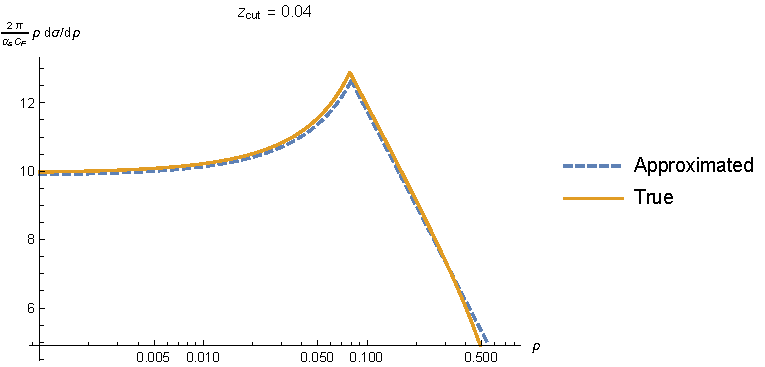
\includegraphics[width=\textwidth]{plots/approximation.pdf}
		\caption{Approximation of the first-order distribution with $\zcut = 0.04$}
	\end{figure}


\bibliographystyle{unsrt}
\bibliography{jet_substructure}

\end{document}